% !TeX root = main.tex
% !TeX spellcheck = de_DE
% !TeX encoding = utf8

\chapter{Implementation}


\section{Simulation}
For simulating the different algorithms I wrote Python scripts. I wrote an encoder using the ALT form. The encoder is a straightforward conversion of the algorithm in \cref{alt_enc_alg} into python code. The code makes heavy use of numpy and scipy for their matrix manipulation abilities. The sparse matrices from the algorithm are also stored as scipy sparse matrices to reduce the memory usage and speed up the encoding process. The overall encoding is split into two parts the offline part done only once and the ending done for every codeword. 

\subsection{Encoder}
The encoder is implemented in 2 different functions. One for the preprocessing where the parity check matrix already in ALT form is split into the required parts and $\Theta$ is inverted. The actual encoding function executes the steps from \cref{p1_steps,p2_steps}. For the sparse matrices $\bm{A}$, $\bm{B}$, $\bm{C}$, $\bm{E}$, and $\bm{T}$ the compressed sparse row matrix format from scipy is used. This format reduced the required memory significantly and accelerates the matrix vector multiplications slightly. 

\subsection{Decoder}
I wrote the decoder to represent the way I planned the FPGA implementation. So the overall structure is doing the steps that the VHDL implementation will also do. I designed it in a way that the python functions that are the core of the decoder roughly map to the VHDL entities. 

\subsubsection{Hardware Overview}
\todo{WTF is this ordering???}
I chose to reduce the hardware complexity by splitting both the check node and the variable node step each into a global calculation and a local one. The global check node calculates \cref{cn_min,cn_min2,cn_min_id,cn_sign} and the local computes \cref{cn_loc}. The same goes for the variable node where the sum over all inputs as in \cref{vn_sum} and then for the local part the input is subtracted \cref{vn_loc}.

\begin{figure}
    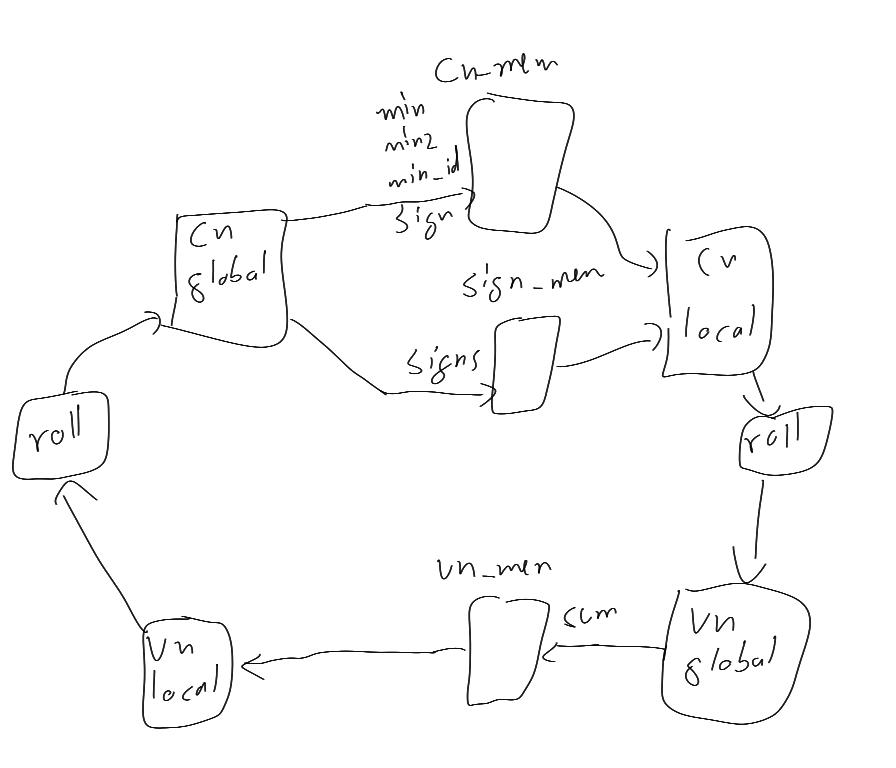
\includegraphics[width=5cm]{dataflow_circle.png}
    put the ugly paper drawing that i have all the time lying around maybe put the sizes of all dem signals here?
    \centering
    \caption{Message and Memory architecture}
\end{figure}

\todo{write something how the thing is done in vivado and u no the block stuff and how the arm cores are used and so on}

\subsection{Results}
The simulation implementation of the decoder is written as a Python script I run them and collect the results. To speed up simulation multiple instances of the script are run in parallel using GNU Parallel. This section lists the bit error rates of the different decoder optimizations.

\subsubsection{Min-sum}
The basic min sum algorithm serves as a baseline for the upcoming improvements. I ran it for two different LDPC codes. Both of them are used by 802.11n for error correction. I chose to use the codes with rate $0.5$ as there is a lot of information available.
\begin{figure}
    \begin{tikzpicture}
        \begin{semilogyaxis}[xlabel={$E_b / N_0$} in dB, ylabel={Error Rate}]
            \addplot table [col sep=tab,x={{Eb/N0 in dB}}, y={FER 648}] {data/sw_err_simple.dat};
            \addlegendentry{FER 648}
            \addplot table [col sep=tab,x={Eb/N0 in dB}, y={BER 648}] {data/sw_err_simple.dat};
            \addlegendentry{BER 648}
            \addplot table [col sep=tab,x={{Eb/N0 in dB}}, y={FER 1944}] {data/sw_err_simple.dat};
            \addlegendentry{FER 1944}
            \addplot table [col sep=tab,x={Eb/N0 in dB}, y={BER 1944}] {data/sw_err_simple.dat};
            \addlegendentry{BER 1944}
        \end{semilogyaxis}
    \end{tikzpicture}
    \centering

    LDPC codes from 802.11n all with rate $0.5$.
    \caption{Frame and Bit Error Rates of the Basic Min Sum Algorithm}
    \label{min_sum_base}
\end{figure}

\subsubsection{Normalized Min-sum}

\begin{figure}
    \begin{tikzpicture}
        \begin{semilogyaxis}[xlabel={$E_b / N_0$} in dB, ylabel={Error Rate}]
            \pgfplotstableread{data/sw_norm_params.dat}\paramopt
            \foreach \x in {1,...,11} {
                \addplot table [col sep=tab,x index={0}, y index={\x}] {\paramopt};
                \pgfplotstablegetcolumnnamebyindex{\x}\of{\paramopt}\to{\colname}
                \addlegendentryexpanded{Normalization \colname}
            }
        \end{semilogyaxis}
    \end{tikzpicture}
    \centering

    \caption{Bit Error Rates of the Normalized Min Sum Algorithm for Different Normalization Factors}
    \label{min_sum_base}
\end{figure}

\subsubsection{Adaptive Normalized Min-sum}
I was not able to improve the performance of the system by using the adaptive normalized min sum algorithm. The performance was on par with the normalized min sum and almost independent of the suppression parameter. 

optimization with more dimensions?

\section{Hardware}
For the hardware implementation an FPGA from Xilinx is used. The device is a "ZYNQ™-7000 SOC XC7Z020-CLG484-1". It in a system on a chip consisting of a dual core ARM processor and programmable logic. The decoder is completely implemented in the FPGA logic and the encoder is software running on the ARM cores. I wrote VHDL code for the encoder.

The parameters for the hardware code were generate using Python scripts.

\subsection{Encoder}
The VHDL implementation for the encoder does the sparse matrix multiplications as fully parallel hardware. All bits are computed in parallel and no intermediate register stages are used as the encoder implemented in this way is faster than required for the decoder anyways. The sparse back substitution of $x^T = \bm{T}y^T$ is done recursively exploiting the advantages of a lower triangular matrix. Any calculation for an output only depends on the inputs and the previously calculated bits. The VHDL code is generated using Python scripts where splitting of the input matrix and the other precomputations are done with the help of numpy. I wrote a simple framework to generate the VHDL code for the matrix multiplications and back substitutions from the precomputed numpy matrices. 

\subsection{Decoder}
\todo{make some block diagramm of all my vhdl entities and their connections}
The decoder is implemented using the algorithm descibed in \cref{chap_approach}. This sections discusses how the algorithm is mapped to a hardware platform. As there are parameters that have to be optimized in oder to get decent decoding performance the decoder is designed in such a way that it is easy to change parameters as for example the bit width of the stored values or the used parity check matrix. 

Overall the decoder is written in VHDL but on file containing definitions for all signals and the decoder state machine is autogenerated with a python script. In this script it is possible to change the bitwidth of the LLRs and the parity check matrix.

The decoder is controlled by a state machine which reads the "instruction list" and outputs the control signal and the memory read and write addresses. This instruction list is also created by the decoder python script. There it is also possible to change the clock cycle in which each signal appears. This makes it easy to change the pipelining. \cref{datafl_tree} shows how the message LLR values are passed along the entities. Each iteration of the decoder is split into two parts. The first part calculated the global check nodes results and the second part the global variable node results.

I will start with the global variable node pass as this has fewer steps and some of the steps are reused in the check node pass. First the local check node results are calculated. This is done from the stored minimum, second minimum, minimum id, and the signs. The output is either the minimum if the minimum id is not equal to the current position or otherwise the second minimum. The sign for this output is taken from the sign input, as all minimums are absolute values. Now the messages are passed through a barrel roll to shift the values to the appropriate positions. The rolled value is then accumulated for each column and at the end of the column stored. 

The global check nodes pass starts the same as the global variable node one until the barrel roll. After rolling the LLRs are passed into the local variable node entity. The local variable node subtracts the incoming LLR from the sums the variable nodes calculated and outputs it. Now the LLRs are passed through a reverse roll to align them for the global check node. The global check node then does an accumulation. This consists of taking the minimum, second minimum, and the signs for the minimum. Also the signs of all incoming LLR values are output.

\begin{figure}
    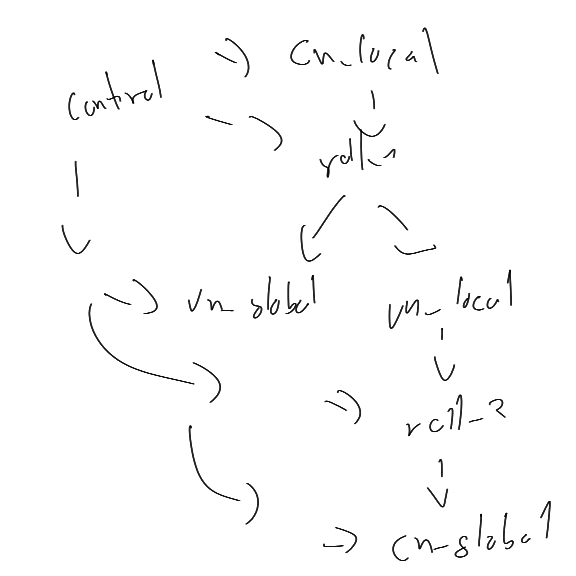
\includegraphics[width=5cm]{dataflow_tree.png}
    maybe add the min mangle at the end
    \centering
    \caption{Dataflow Diagram of the Decoder}
    \label{datafl_tree}
\end{figure}

\subsection{Control}
The decoder is controlled by a state machine which reads the addresses for the memory and all control signals from a ROM. It als keeps track of the number of iterations already done and terminates if the iteration number reaches a specified maximum. Additionally the state machine stops the decoding process if the output vector is error free. The instructions consisting of addresses and control signal are generated by the Python script which also generates the other constants. In my script to generate the instructions I \todo{continue with something about how great my fucking subroutine with a weee bit of string manipulation is}

\subsection{Check Nodes}
As the check nodes are split into two steps I wrote two separate entities executing these operations. One is the local check node, computes the message LLR from the minimums, minimum sign, and LLR signs. From the controller it receives the current offset. 

\begin{figure}
    LLR from min schematic maybe?
    \centering
    \caption{Schematic Diagram of a Local Check Node}
\end{figure}

\begin{figure}
    min entity schematic maybe?
    \centering
    \caption{Schematic Diagram of a Global Check Node}
\end{figure}

\subsection{Variable Nodes}
Also the variable nodes are split into two. The global pass sums all the incoming LLR values and at the end of each column it is stored into memory. The local check node retrieves these sums and calculates
\begin{equation}
    q_{nm} = S(n) - r_{mn}
\end{equation}
, where $S(n)$ is the stored column sum, $r_{mn}$ and $q_{nm}$ are the incoming and outgoing LLRs respectively.

\subsection{Barrel Roll}
I started first with a naive implementation for the barrel roll
\begin{lstlisting}[style=vhdl]
    entity dynamic_roll_sign is
	generic (
		DIRECTION : boolean --true means the same direction as fixed roll
	);
    port (
		roll_count : in unsigned;
        data_in : in min_signs_t;
		data_out : out min_signs_t
    );
end entity;

architecture base of dynamic_roll_sign is
begin
    gen_i : for i in data_in'range generate
    begin
        data_out(i) <= data_in((i - to_integer(roll_count)) mod data_in'length) when not DIRECTION 
            else data_in((i + to_integer(roll_count)) mod data_in'length));
    end generate;
end architecture;
\end{lstlisting}
but this generates huge hardware. The primary problem is the synthesis generates a division to implement the modulo operations. In the following I will show that the modulo can in this case be replaced by a conditional addition or subtraction. But first I have to set some limits for the inputs. I only allow roll values in the range $0 \leq$ \lstinline{roll_count} $<$ \lstinline{data_in'length}. From that and the possible values for $i$ I get $0 \leq + $ \lstinline{roll_count} $ < 2$ \lstinline{data_in'length}. Knowing this I can replace the modulo with a conditional addition or subtraction depending on the shift direction. So the lines writing to \lstinline{data_out} are replaced by:
\begin{lstlisting}
data_out(i, j) <= data_in(add_mod(i - to_integer(roll_count), data_in'length), j) when not DIRECTION 
    else data_in(sub_mod(i + to_integer(roll_count), data_in'length), j);
\end{lstlisting}

\begin{table}
    \begin{tabular}{l r r}
        %roll_2 resource utilization with block length 27 and 200
        Algorithm & 27 Block Length & 200 Block Length \\ \toprule
        Modulo & 5132 & 101533 \\
        Sub & 540 &  28229\\
        MUX2 & 473 & 5600
    \end{tabular}
    \centering
    \caption{LUT Utilization of Different Barrel Roll Implementations}
    \label{roll_usage}
\end{table}

Even more efficient in resource usage is a logarithmic barrel shifter. In this design I have shifts by powers of two and either use each shift or bypass it depending on the \lstinline{roll_count} bits. In \cref{log_shift} you can see a block diagram of such an architecture. This design only requires wires and two input muxes. On the used FPGA each LUT can implement a 4 input LUT or multiple LUTs can work together to create muxes with more inputs. I tried the architecture with larger muxes but archived no smaller design. This optimization was probably already done by the synthesis tools and doing it manually did not change the resource usage. The differece between the barrel shifters is more pronounced at larger block sizes as is visible in \cref{roll_usage}.\todo{requrce usage!!}

In \cref{roll_usage} you can see that for the block length of 200 it is not feasible to use the worse algorithm. And modern codes such as one proposed for NG-EPON\cite{wey_3ca_1a_0118} and DVB-S2\cite{ETSI_EN_302_307}.

\begin{figure}
    \tikzstyle{branch}=[fill,shape=circle,minimum size=3pt,inner sep=0pt]
    \begin{tikzpicture}[x=1.5cm,y=2cm]
        \foreach \x in {0,...,7} {
            \node (r\x) at (\x, 0) {in[\x]};
            \node (u\x) at (\x, -3.5) {out[\x]};
            \foreach \y [evaluate=\y as \yn using int(\y-1), evaluate=\x as \xpow using {int(round(Mod(\x+\y,8)))}] in {1,2,3} {
                \pgfmathsetmacro{\xsh}{int(round(Mod(\x+2^(0),8)))}
                \pgfmathsetmacro{\poff}{(\x+1) /9}
                \ifnum\x=1
                    \node at (-1.5,-\y) {roll\_count[\y]};
                \fi
                \node (n\x\y) [draw, minimum width=1cm] at (\x, -\y) {MUX};
                \ifnum\y=1
                    
                    \draw ($(r\x.south)+(0.3cm,0)$) -- ($(n\x\y.north)+(0.3cm,0)$) node [pos=\poff,branch] (m\x\y) {};
                \else
                    \ifnum\y=3
                        \draw($(n\x\y.south)+(0.3cm,0)$) -- ($(u\x.north)+(0.3cm,0)$);
                    \fi
                    \draw ($(n\x\yn.south)+(0.3cm,0)$) -- ($(n\x\y.north)+(0.3cm,0)$)  node [pos=\poff,branch] (m\x\y) {};
                \fi
            }
        }
        \foreach \x in {0,...,7} {
            \pgfmathsetmacro{\xsh}{int(round(Mod(\x+2^(0),8)))}
            \foreach \y [evaluate=\y as \yn using int(\y-1), evaluate=\x as \xpow using {int(round(Mod(\x-2^(\y-1),8)))}] in {1,2,3} {
                \draw ($(n\x\y.north)+(-0.3cm,0)$) |- (m\xpow\y.center);
            }
        }
    \end{tikzpicture}
    \centering
    \caption{Structure of a Logarithmic Barrel Shifter}
    \label{log_shift}
\end{figure}

\subsection{Interface}
I used AXI-Stream interfaces to input the LLR values into the decoder and to output the decoded bits. These interfaces transfer the bits tightly packed to maximize throughput. The stream interface is a good fit for this application as decoding is done on full frames and the is no need to change single words after a transfer. Also it is fast to implement.

\subsection{Pipelining}
If implemented without any pipeline steps the maximum clock for the 648 bits message length, rate $0.5$, and 7 bit LLR is ~27Mhz\todo{check real val}. By adding registers between some steps I reduce the critical path. By adding two stages I increase the maximum clock rate to ~70Mhz\todo{test}. The pipeline stages are added between the local check node and the first barrel roll and after the second barrel roll. These position were determined by check the critical path timing in Vivado and adding registers to achieve a maximum critical path length of 10ns as to get a 100Mhz clock. \todo{i prolly need one after the global check node to get the memory timing better}

\subsection{Possible Improvements}
More pipelining
In and output double buffering
More pipeline stages
u no dependency optimization

\section{Data Source}
For evaluating the whole pipeline a source of data to be encoded is required. I used a uniform random number generator. The numbers were generated using a Tausworthe generator\cite{Ec96}. I implemented it in a straightforward manner in VHDL. There were no difficulties as it consists of static shifts and bit boolean operators.

\section{Channel Model}
To test an error correction scheme a source of errors is required. This would usually be the flash memory in an solid state drive, but here I simulate it using gaussian noise. The gaussian noise is generated with the Box-Muller method using the hardware approach from Dong-U Lee, John D. Villasenor and Wayne Luk and Philip H. W. Leong\cite{LeVi06}. Here I used Vivado HLS to create the hardware. The Box-Muller method requires fixed point numbers and with high level synthesis it is very fast to write the code for such a noise generator.

My tests concluded the Box Muller method is to hardware intensive when build with high level synthesis. I used a very efficient design by David B. Thomas\cite{Th14} which uses less resources of the FPGA. The class of gaussian number generators described in Thomas paper have different qualities depending on the internal bitwidths. I chose the one with the highest quality as it is still smaller than my Box-Muller implementation. To interface with my existing design I wrote an axi stream frontend to simply replace the other number generator. The Box-Muller method used for example 6845 LUTs compared to ~683 LUTs for this method. The output from the generator is a 26 bit fixed point number with 6 bit integer part.

\section{LLR Conversion}
The LLR calculation is done as descibed in \cref{llr_approach}. The hardware block for the LLR takes $y_i$ and $\frac{2}{\sigma^2}$ is precomputed on the ARM core and then sent as a 32 bit fixed point number with 5 bit integer part to the programmable system. The result of this conversion is then rounded to the number of bits the encoder is using.

\section{Result Accumulation}
The results of each decoding are compared to the input to the channel. As the output of the decoder is a 32 bit axi stream multiple word have to be compared for each decoding. The Hamming distance between the expected and decoded codeword is then sent to ARM core.

\section{Control}
The whole system is controlled by the ARM core of the SoC. The parameters of the test system are set first by the ARM and then the encoder decoder core is set to run. While it is running the bit error counts of each transmission are read out and summed. As each frame is handled separately by the result accumulator a frame error can be detected easily by checking if the bit error count for a frame differs from zero. This split in functionality simplifies testing for different parameters enormously because new software for the cpu can be written and compiled very quickly compared to synthesizing VHDL code for the FPGA part.

circuitry
